\documentclass[journal,12pt,twocolumn]{IEEEtran}
\usepackage{amsmath,amsfonts,amssymb,float}
\usepackage{graphicx}
\bibliographystyle{IEEEtran}
\vspace{3cm}
\title{NCERT Discrete}
\author{Pragnidhved Reddy\\EE23BTECH11050}
\date{}
\parindent 0px
\begin{document}
\maketitle
\newpage
\bigskip
\textbf{Question 10.5.2.8:}\\
An AP consists of $50$ terms of which $3^{rd}$ term is $12$ and the last term is $106$. Find the $29^{th}$ term.\\
\textbf{Solution :}\\
\begin{table}[H]
\centering
\begin{tabular}{|c|c|c|}\hline
\textbf{Parameter} & \textbf{Value} & \textbf{description}\\ \hline
$x(0)$ & $6$ & First term\\ \hline
$d$ & $2$ & common difference\\ \hline
$x(n)$ & $[x(0)+2n]u(n)$ & general term \\ \hline
\end{tabular}
\caption{Input parameters}
\end{table}
In this AP we can tell that x(0)=6.\\
Therefore, x(n)=6+2n.
$$X(z)=\frac{6-8z^{-1}}{(1-z^{-1})^2} \quad \abs{z}>1$$
\begin{figure}[h!]
    \centering
    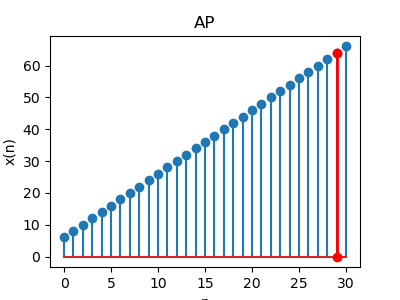
\includegraphics{figs/plot.png}
    \caption{graph of the given AP}
    \label{fig:1}
\end{figure}
\end{document}
